% Generated by code/needham.py -- do not edit by hand.
\definecolor{qocA}{rgb}{0.00,0.45,0.70}
\definecolor{qocB}{rgb}{0.90,0.60,0.00}
\definecolor{qocC}{rgb}{0.00,0.62,0.45}
\definecolor{qocD}{rgb}{0.80,0.40,0.00}
\definecolor{qocE}{rgb}{0.80,0.60,0.70}
\definecolor{qocF}{rgb}{0.35,0.70,0.90}
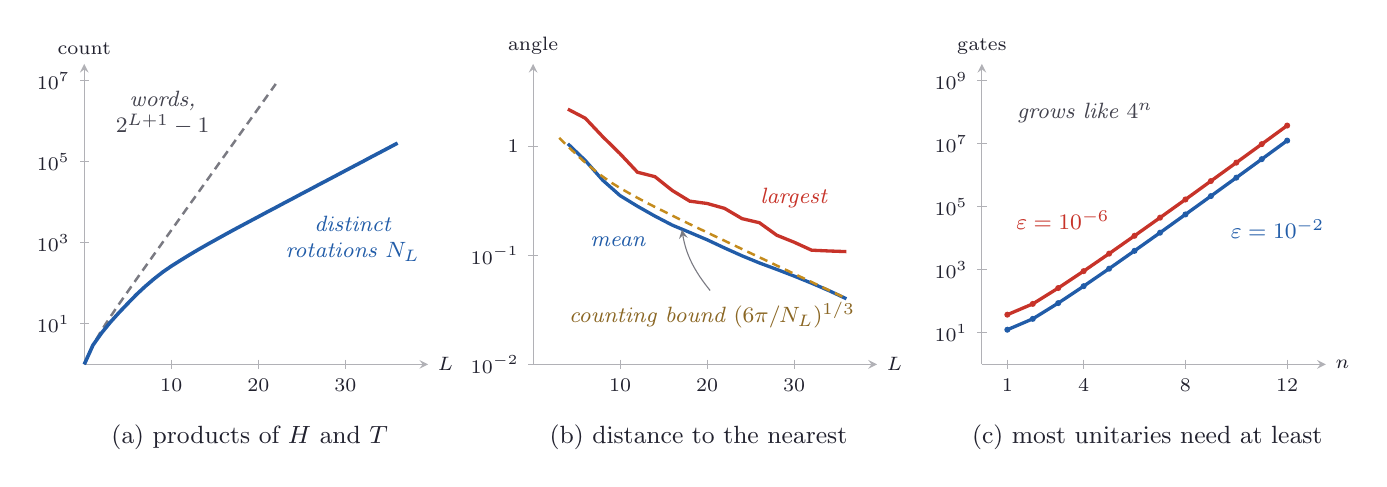
\begin{tikzpicture}[ink/.style={line width=0.9pt, ndInk}, faint/.style={line width=0.4pt, ndInk!35}, dashedink/.style={line width=0.5pt, ndInk!55, dash pattern=on 2.5pt off 2pt}, vec/.style={->, >=stealth, line width=1.2pt}, note/.style={font=\footnotesize\itshape, text=ndInk!85, align=center}, pointer/.style={->, >=stealth, line width=0.4pt, ndInk!60, shorten >=2pt, shorten <=1pt}, dot/.style={circle, fill=ndInk, inner sep=0pt, minimum size=3.4pt}, wash/.style={fill=ndSky, fill opacity=0.55}, every node/.style={text=ndInk}]
\definecolor{ndInk}{rgb}{0.13,0.13,0.18}
\definecolor{ndPaper}{rgb}{0.99,0.96,0.88}
\definecolor{ndSky}{rgb}{0.84,0.91,0.98}
\definecolor{ndRose}{rgb}{0.98,0.86,0.84}
\definecolor{ndBlue}{rgb}{0.13,0.36,0.66}
\definecolor{ndRed}{rgb}{0.78,0.20,0.16}
\definecolor{ndGold}{rgb}{0.88,0.62,0.10}
\definecolor{ndGreen}{rgb}{0.18,0.52,0.30}
\draw[faint, ->, >=stealth] (0.900,0.700) -- (5.268,0.700) node[right, text=ndInk] {{\scriptsize $L$}};
\draw[faint, ->, >=stealth] (0.900,0.700) -- (0.900,4.516) node[above, text=ndInk] {{\scriptsize count}};
\draw[faint] (2.005,0.760) -- (2.005,0.640) node[below, font=\scriptsize, text=ndInk] {$10$};
\draw[faint] (3.111,0.760) -- (3.111,0.640) node[below, font=\scriptsize, text=ndInk] {$20$};
\draw[faint] (4.216,0.760) -- (4.216,0.640) node[below, font=\scriptsize, text=ndInk] {$30$};
\draw[faint] (0.960,1.214) -- (0.840,1.214) node[left, font=\scriptsize, text=ndInk] {$10^{1}$};
\draw[faint] (0.960,2.243) -- (0.840,2.243) node[left, font=\scriptsize, text=ndInk] {$10^{3}$};
\draw[faint] (0.960,3.271) -- (0.840,3.271) node[left, font=\scriptsize, text=ndInk] {$10^{5}$};
\draw[faint] (0.960,4.300) -- (0.840,4.300) node[left, font=\scriptsize, text=ndInk] {$10^{7}$};
\draw[line width=0.9pt, ndInk!60, dash pattern=on 3pt off 2pt] (0.900,0.700) -- (1.011,0.945) -- (1.121,1.135) -- (1.232,1.305) -- (1.342,1.467) -- (1.453,1.625) -- (1.563,1.782) -- (1.674,1.938) -- (1.784,2.093) -- (1.895,2.248) -- (2.005,2.403) -- (2.116,2.558) -- (2.226,2.713) -- (2.337,2.867) -- (2.447,3.022) -- (2.558,3.177) -- (2.668,3.332) -- (2.779,3.487) -- (2.889,3.641) -- (3.000,3.796) -- (3.111,3.951) -- (3.221,4.106) -- (3.332,4.261);
\draw[line width=1.3pt, ndBlue] (0.900,0.700) -- (1.011,0.945) -- (1.121,1.100) -- (1.232,1.236) -- (1.342,1.358) -- (1.453,1.474) -- (1.563,1.587) -- (1.674,1.690) -- (1.784,1.784) -- (1.895,1.871) -- (2.005,1.947) -- (2.116,2.017) -- (2.226,2.085) -- (2.337,2.151) -- (2.447,2.214) -- (2.558,2.276) -- (2.668,2.337) -- (2.779,2.398) -- (2.889,2.457) -- (3.000,2.516) -- (3.111,2.575) -- (3.221,2.634) -- (3.332,2.692) -- (3.442,2.751) -- (3.553,2.809) -- (3.663,2.868) -- (3.774,2.926) -- (3.884,2.985) -- (3.995,3.043) -- (4.105,3.101) -- (4.216,3.160) -- (4.326,3.218) -- (4.437,3.276) -- (4.547,3.335) -- (4.658,3.393) -- (4.768,3.451) -- (4.879,3.510);
\node[note, anchor=east] at (2.613,3.889) {words,\\ $2^{L+1}-1$};
\node[note, anchor=north west, text=ndBlue] at (3.332,2.706) {distinct\\ rotations $N_L$};
\node[font=\small, anchor=north] at (3.000,0.057) {(a) products of $H$ and $T$};
\draw[faint, ->, >=stealth] (6.600,0.700) -- (10.968,0.700) node[right, text=ndInk] {{\scriptsize $L$}};
\draw[faint, ->, >=stealth] (6.600,0.700) -- (6.600,4.516) node[above, text=ndInk] {{\scriptsize angle}};
\draw[faint] (7.705,0.760) -- (7.705,0.640) node[below, font=\scriptsize, text=ndInk] {$10$};
\draw[faint] (8.811,0.760) -- (8.811,0.640) node[below, font=\scriptsize, text=ndInk] {$20$};
\draw[faint] (9.916,0.760) -- (9.916,0.640) node[below, font=\scriptsize, text=ndInk] {$30$};
\draw[faint] (6.660,0.700) -- (6.540,0.700) node[left, font=\scriptsize, text=ndInk] {$10^{-2}$};
\draw[faint] (6.660,2.085) -- (6.540,2.085) node[left, font=\scriptsize, text=ndInk] {$10^{-1}$};
\draw[faint] (6.660,3.469) -- (6.540,3.469) node[left, font=\scriptsize, text=ndInk] {$1$};
\draw[line width=1.2pt, ndRed] (7.042,3.941) -- (7.263,3.826) -- (7.484,3.592) -- (7.705,3.375) -- (7.926,3.140) -- (8.147,3.084) -- (8.368,2.908) -- (8.589,2.773) -- (8.811,2.743) -- (9.032,2.681) -- (9.253,2.551) -- (9.474,2.499) -- (9.695,2.340) -- (9.916,2.251) -- (10.137,2.150) -- (10.358,2.140) -- (10.579,2.132);
\draw[line width=1.2pt, ndBlue] (7.042,3.501) -- (7.263,3.289) -- (7.484,3.039) -- (7.705,2.843) -- (7.926,2.708) -- (8.147,2.583) -- (8.368,2.468) -- (8.589,2.376) -- (8.811,2.282) -- (9.032,2.178) -- (9.253,2.079) -- (9.474,1.988) -- (9.695,1.906) -- (9.916,1.821) -- (10.137,1.731) -- (10.358,1.636) -- (10.579,1.533);
\draw[line width=0.9pt, ndGold!85!ndInk, dash pattern=on 3pt off 2pt] (6.932,3.577) -- (7.042,3.468) -- (7.153,3.363) -- (7.263,3.262) -- (7.374,3.170) -- (7.484,3.085) -- (7.595,3.007) -- (7.705,2.939) -- (7.816,2.876) -- (7.926,2.815) -- (8.037,2.756) -- (8.147,2.699) -- (8.258,2.644) -- (8.368,2.589) -- (8.479,2.534) -- (8.589,2.481) -- (8.700,2.428) -- (8.811,2.375) -- (8.921,2.322) -- (9.032,2.270) -- (9.142,2.217) -- (9.253,2.165) -- (9.363,2.112) -- (9.474,2.060) -- (9.584,2.008) -- (9.695,1.955) -- (9.805,1.903) -- (9.916,1.850) -- (10.026,1.798) -- (10.137,1.746) -- (10.247,1.693) -- (10.358,1.641) -- (10.468,1.589) -- (10.579,1.536);
\node[note, anchor=south west, text=ndRed] at (9.363,2.568) {largest};
\node[note, anchor=north east, text=ndBlue] at (8.147,2.444) {mean};
\node[note, anchor=west, text=ndGold!55!ndInk] (bd) at (6.932,1.323) {counting bound $(6\pi/N_L)^{1/3}$};
\draw[pointer] (bd.north) to[bend left=15] (8.479,2.479);
\node[font=\small, anchor=north] at (8.700,0.060) {(b) distance to the nearest};
\draw[faint, ->, >=stealth] (12.300,0.700) -- (16.668,0.700) node[right, text=ndInk] {{\scriptsize $n$}};
\draw[faint, ->, >=stealth] (12.300,0.700) -- (12.300,4.516) node[above, text=ndInk] {{\scriptsize gates}};
\draw[faint] (12.623,0.760) -- (12.623,0.640) node[below, font=\scriptsize, text=ndInk] {$1$};
\draw[faint] (13.592,0.760) -- (13.592,0.640) node[below, font=\scriptsize, text=ndInk] {$4$};
\draw[faint] (14.885,0.760) -- (14.885,0.640) node[below, font=\scriptsize, text=ndInk] {$8$};
\draw[faint] (16.177,0.760) -- (16.177,0.640) node[below, font=\scriptsize, text=ndInk] {$12$};
\draw[faint] (12.360,1.100) -- (12.240,1.100) node[left, font=\scriptsize, text=ndInk] {$10^{1}$};
\draw[faint] (12.360,1.900) -- (12.240,1.900) node[left, font=\scriptsize, text=ndInk] {$10^{3}$};
\draw[faint] (12.360,2.700) -- (12.240,2.700) node[left, font=\scriptsize, text=ndInk] {$10^{5}$};
\draw[faint] (12.360,3.500) -- (12.240,3.500) node[left, font=\scriptsize, text=ndInk] {$10^{7}$};
\draw[faint] (12.360,4.300) -- (12.240,4.300) node[left, font=\scriptsize, text=ndInk] {$10^{9}$};
\draw[line width=1.2pt, ndBlue] (12.623,1.140) -- (12.946,1.278) -- (13.269,1.478) -- (13.592,1.693) -- (13.915,1.915) -- (14.238,2.142) -- (14.562,2.372) -- (14.885,2.604) -- (15.208,2.837) -- (15.531,3.071) -- (15.854,3.306) -- (16.177,3.542);
\node[circle, fill=ndBlue, inner sep=0pt, minimum size=2.2pt] at (12.623,1.140) {};
\node[circle, fill=ndBlue, inner sep=0pt, minimum size=2.2pt] at (12.946,1.278) {};
\node[circle, fill=ndBlue, inner sep=0pt, minimum size=2.2pt] at (13.269,1.478) {};
\node[circle, fill=ndBlue, inner sep=0pt, minimum size=2.2pt] at (13.592,1.693) {};
\node[circle, fill=ndBlue, inner sep=0pt, minimum size=2.2pt] at (13.915,1.915) {};
\node[circle, fill=ndBlue, inner sep=0pt, minimum size=2.2pt] at (14.238,2.142) {};
\node[circle, fill=ndBlue, inner sep=0pt, minimum size=2.2pt] at (14.562,2.372) {};
\node[circle, fill=ndBlue, inner sep=0pt, minimum size=2.2pt] at (14.885,2.604) {};
\node[circle, fill=ndBlue, inner sep=0pt, minimum size=2.2pt] at (15.208,2.837) {};
\node[circle, fill=ndBlue, inner sep=0pt, minimum size=2.2pt] at (15.531,3.071) {};
\node[circle, fill=ndBlue, inner sep=0pt, minimum size=2.2pt] at (15.854,3.306) {};
\node[circle, fill=ndBlue, inner sep=0pt, minimum size=2.2pt] at (16.177,3.542) {};
\draw[line width=1.2pt, ndRed] (12.623,1.331) -- (12.946,1.468) -- (13.269,1.669) -- (13.592,1.884) -- (13.915,2.106) -- (14.238,2.333) -- (14.562,2.563) -- (14.885,2.794) -- (15.208,3.028) -- (15.531,3.262) -- (15.854,3.497) -- (16.177,3.733);
\node[circle, fill=ndRed, inner sep=0pt, minimum size=2.2pt] at (12.623,1.331) {};
\node[circle, fill=ndRed, inner sep=0pt, minimum size=2.2pt] at (12.946,1.468) {};
\node[circle, fill=ndRed, inner sep=0pt, minimum size=2.2pt] at (13.269,1.669) {};
\node[circle, fill=ndRed, inner sep=0pt, minimum size=2.2pt] at (13.592,1.884) {};
\node[circle, fill=ndRed, inner sep=0pt, minimum size=2.2pt] at (13.915,2.106) {};
\node[circle, fill=ndRed, inner sep=0pt, minimum size=2.2pt] at (14.238,2.333) {};
\node[circle, fill=ndRed, inner sep=0pt, minimum size=2.2pt] at (14.562,2.563) {};
\node[circle, fill=ndRed, inner sep=0pt, minimum size=2.2pt] at (14.885,2.794) {};
\node[circle, fill=ndRed, inner sep=0pt, minimum size=2.2pt] at (15.208,3.028) {};
\node[circle, fill=ndRed, inner sep=0pt, minimum size=2.2pt] at (15.531,3.262) {};
\node[circle, fill=ndRed, inner sep=0pt, minimum size=2.2pt] at (15.854,3.497) {};
\node[circle, fill=ndRed, inner sep=0pt, minimum size=2.2pt] at (16.177,3.733) {};
\node[note, anchor=south east, text=ndRed] at (14.045,2.286) {$\varepsilon=10^{-6}$};
\node[note, anchor=north west, text=ndBlue] at (15.337,2.657) {$\varepsilon=10^{-2}$};
\node[note, anchor=north west] at (12.623,4.140) {grows like $4^n$};
\node[font=\small, anchor=north] at (14.400,0.060) {(c) most unitaries need at least};
\end{tikzpicture}
